\section{Design}
\label{sec:Design}

The focal length and dimension of each lens had to be identified to determine which combination of lenses would make the best telescope. The focal lengths of four lenses were experimentally measured by using the sun as a light source. We approximated the sun to be an infinite distance away, producing nearly parallel rays. We focused the lenses until they produced a single dot of light on the bottom of a metal support stand. The distance from the lens to the bottom of the stand was measured with rulers while the lens was tightly clamped at the focused position. This experiment had an error of $\pm$ \SI{0.1}{\centi\meter}. The diameters of the lenses were measured using Vernier calipers which had an error of $\pm$ \SI{0.05}{\milli\meter}. 

\subsection{Choice of Lenses}

\begin{table}[!h]
  \begin{center}
    \caption{Lens Profiles} \label{lens_iden}
    \setlength\tabcolsep{1.5em}
    \begin{tabular}{c c c c}
      \hline \hline 
      \multicolumn{1}{c}{\bf (1)} &
      \multicolumn{1}{c}{\bf (2)} &
      \multicolumn{1}{c}{\bf (3)} &
      \multicolumn{1}{c}{\bf (4)} \\
      \bigbreak
      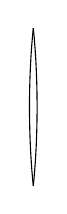
\begin{tikzpicture}[xscale = 0.18][yscale=2]
        \pgfmathsetmacro{\lensRadius}{2}
        \pgfmathsetmacro{\lensHeight}{1}
        \pgfmathsetmacro{\startAngle}{asin(\lensHeight/\lensRadius)}
        \draw (0,\lensHeight) arc[start angle=180-\startAngle,delta angle=2*\startAngle,radius=\lensRadius];
        \draw (0,\lensHeight) arc[start angle=\startAngle,delta angle=-2*\startAngle,radius=\lensRadius];
      \end{tikzpicture} &
      
      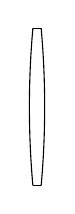
\begin{tikzpicture}[xscale = 0.35][yscale=2]
        \pgfmathsetmacro{\lensRadius}{4}
        \pgfmathsetmacro{\lensHeight}{1}
        \pgfmathsetmacro{\startAngle}{asin(\lensHeight/\lensRadius)}
        \draw (0,\lensHeight) arc[start angle=180-\startAngle,delta angle=2*\startAngle,radius=\lensRadius];
        \draw (0.3,\lensHeight) arc[start angle=\startAngle,delta angle=-2*\startAngle,radius=\lensRadius];
        \draw[-] (0,1) -- (0.3,1);
        \draw[-] (0,-1) -- (0.3,-1);
      \end{tikzpicture} &

      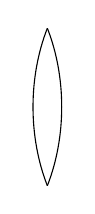
\begin{tikzpicture}[xscale = 0.68][yscale=2]
        \pgfmathsetmacro{\lensRadius}{2}
        \pgfmathsetmacro{\lensHeight}{1}
        \pgfmathsetmacro{\startAngle}{asin(\lensHeight/\lensRadius)}
        \draw (0,\lensHeight) arc[start angle=180-\startAngle,delta angle=2*\startAngle,radius=\lensRadius];
        \draw (0,\lensHeight) arc[start angle=\startAngle,delta angle=-2*\startAngle,radius=\lensRadius];
      \end{tikzpicture} &

      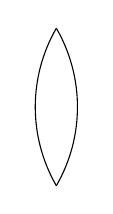
\begin{tikzpicture}[xscale = 1][yscale=2]
        \pgfmathsetmacro{\lensRadius}{2}
        \pgfmathsetmacro{\lensHeight}{1}
        \pgfmathsetmacro{\startAngle}{asin(\lensHeight/\lensRadius)}
        \draw (0,\lensHeight) arc[start angle=180-\startAngle,delta angle=2*\startAngle,radius=\lensRadius];
        \draw (0,\lensHeight) arc[start angle=\startAngle,delta angle=-2*\startAngle,radius=\lensRadius];
      \end{tikzpicture} \\
    \end{tabular}
  \end{center}
\end{table}

\vspace*{-\baselineskip} %Removes excessive spacing
\vspace*{-\baselineskip} %Removes excessive spacing
%\vspace*{-\baselineskip} %Removes excessive spacing

\begin{table}[!h]
  \begin{center}
    \caption{Lens Specifications.} \label{lens_specs}
    %\bigbreak
    \begin{tabular}{l | l | l}
      \hline \hline
      \multicolumn{1}{l}{\bf Identification} &
      \multicolumn{1}{l}{\bf Focal Length} &
      \multicolumn{1}{l}{\bf Diameter} \\
      \hline
      (1) & \SI{50.3}{\centi\meter} & \SI{49.16}{\milli\meter} \\
      (2) & \SI{25.9}{\centi\meter} & \SI{49.79}{\milli\meter} \\
      (3) & \SI{9.60}{\centi\meter} & \SI{50.35}{\milli\meter} \\
      (4) & \SI{5.40}{\centi\meter} & \SI{50.00}{\milli\meter} \\
      %\hline \hline
    \end{tabular}
  \end{center}
\end{table}

Table I shows the profile of the lenses relative to each other and how they were numbered. From now on, we will refer to the lenses using this numbering. Table II provides the dimensions of each lens. 

\begin{figure}[!h]
  \begin{center}
    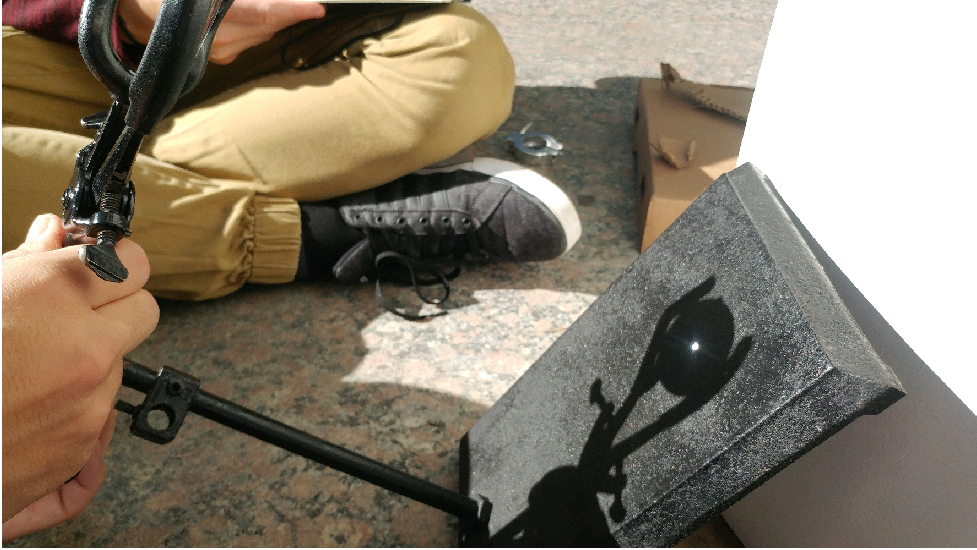
\includegraphics[width=0.3\textwidth]{./Figures/focal_length.pdf}
    \caption{Set up used to determine focal length.}
  \end{center}
\end{figure}

Two lenses were selected based on comparisons of effective magnification, clarity, and practicality in telescope length. The length of the telescope must be equal to the sum of the focal lengths of the chosen lenses in order to form a magnified image \cite{tb}. The length also needed to remain within the dimension limits of the 3D printer. Keeping these requirements in mind, we immediately eliminated lens (1) as a potential candidate due to its relatively large focal length. If this lens were to be used, the telescope would be long enough to produce a bowing effect, misaligning the lenses and preventing image formation. Further, the focal length would have pushed the telescope’s dimensions outside the printable range. Aside from length limitations, lens (1) has a larger $f$-number than lens (2). A larger $f$-number produces a dimmer and less clear image \cite{tb}. $f$-number is calculated from the following equation
\[f\text{-number} = \dfrac{f}{D}\]
where $f$ is the focal length of the lens and $D$ is the diameter of the lens. Since the diameters of the lenses are approximately equal, the $f$-number of lens (1) is about two times that of lens (2). We eliminated lens (4) due to its odd geometry, which would add unnecessary difficulty while printing. This leaves lenses (2) and (3). Lens (2) is the objective lens and lens (3) is the eyepiece. This combination offered a good balance between clarity and telescope length.

\subsection{Theory}

The sum the focal lengths of lens (2) and lens (3) gives us a theoretical telescope length of \SI{35.5}{\centi\meter}. The angular magnification of the telescope can be calculated using the equation
\begin{equation}\label{mag}
  M=-\dfrac{f_1}{f_2}
\end{equation}
where $f_1$ is the focal length of the objective lens and $f_2$ is the focal length of the eyepiece lens. The theoretical magnification is \SI{2.70}{}x. 

%\bigbreak

\begin{figure}[!h]
\begin{adjustwidth}{-1.5cm}{}
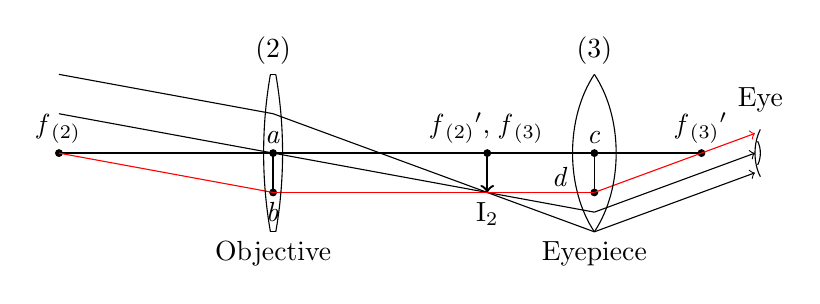
\begin{tikzpicture}[xscale = 0.68][yscale=2]
  \coordinate (x) at (0,0);
  \node at (x) {};
  \coordinate (y) at (12,0);
  \node at (y) {};
  \draw[line width=0.2mm] (x) -- (y);
  \coordinate (a) at (4,0);
  \node[above] at (a) {\textit{a}}; 
  \fill[shift only](a) circle [radius=.5mm];
  \coordinate (b) at (4,-0.5);
  \node[below] at (b) {\textit{b}}; 
  \fill[shift only](b) circle [radius=.5mm];
  \coordinate (c) at (10,0);
  \node[above] at (c) {\textit{c}};
  \fill[shift only](c) circle [radius=.5mm];
  \coordinate (d) at (10,-0.5);
  \node[above = 2mm, left = 2mm] at (d) {\textit{d}}; 
  \fill[shift only](d) circle [radius=.5mm];
  \draw[line width=0.2mm] (a) -- (b);
  \draw[line width=0.2mm] (c) -- (d);
  %--- Image
  \coordinate (ix) at (8,0);
  \coordinate (i) at (8,-0.5);
  \node[below] at (i) {I\textsubscript{2}};
  \node[above] at (ix) {\textit{f}\textsubscript{(2)}$'$, \textit{f}\textsubscript{(3)}};
  \fill[shift only](ix) circle [radius=.5mm];
  \draw[line width = 0.3mm, ->] (ix) -- (i);
  %--- Focal Points
  \coordinate (f1) at (0,0);
  \node[above] at (f1){\textit{f}\textsubscript{(2)}};
  \fill[shift only](f1) circle [radius=.5mm];
  \coordinate (f2) at (12,0);
  \node[above] at (f2){\textit{f}\textsubscript{(3)}$'$};
  \fill[shift only](f2) circle [radius=.5mm];
  %---Rays
  \draw[] (0,1) -- (4,0.5);
  \draw[] (0,0.5) -- (4,0);
  \draw[red] (x) -- (b);
  
  \draw[] (4,0.5) -- (10,-1);
  \draw[] (4,0) -- (10,-0.75);
  \draw[red] (4,-0.5) -- (10,-0.5);
  
  \draw[->] (10,-1) -- (13,-0.25);
  \draw[->] (10,-0.75) -- (13,-0);
  \draw[red, ->] (10,-0.5) -- (13,0.25);
  \coordinate (p) at (13.1,0);
  \node[above = 4mm] at (p){Eye};
  %\fill[shift only](p) circle [radius=1mm];
  \pgfmathsetmacro{\lensRadius}{0.5}
  \pgfmathsetmacro{\lensHeight}{0.3}
  \pgfmathsetmacro{\startAngle}{asin(\lensHeight/\lensRadius)}
  \draw (13.1,\lensHeight) arc[start angle=180-\startAngle,delta angle=2*\startAngle,radius=\lensRadius];
%  \draw (13,\lensHeight) arc[start angle=180-\startAngle,delta angle=2*\startAngle,radius=\lensRadius];
  \draw (13.05,0.15) arc[start angle=\startAngle,delta angle=-2*\startAngle,radius=\lensRadius/2];  
  %--- Lenses
  \pgfmathsetmacro{\lensRadius}{4}
  \pgfmathsetmacro{\lensHeight}{1}
  \pgfmathsetmacro{\startAngle}{asin(\lensHeight/\lensRadius)}
  \draw (3.95,\lensHeight) arc[start angle=180-\startAngle,delta angle=2*\startAngle,radius=\lensRadius];
  \draw (4.05,\lensHeight) arc[start angle=\startAngle,delta angle=-2*\startAngle,radius=\lensRadius];
  \draw[-] (3.95,1) -- (4.05,1);
  \draw[-] (3.95,-1) -- (4.05,-1);
  \node[below] at (4,-1){Objective};
  \node[above] at (4,1){(2)};
  \pgfmathsetmacro{\lensRadius}{1.43}
  \pgfmathsetmacro{\lensHeight}{1}
  \pgfmathsetmacro{\startAngle}{asin(\lensHeight/\lensRadius)}
  \draw (10,\lensHeight) arc[start angle=180-\startAngle,delta angle=2*\startAngle,radius=\lensRadius];
  \draw (10,\lensHeight) arc[start angle=\startAngle,delta angle=-2*\startAngle,radius=\lensRadius];
  \node[below] at (10,-1){Eyepiece};
  \node[above] at (10,1){(3)};
\end{tikzpicture}
\caption{Ray diagram}
\label{fig:ray}
\end{adjustwidth}
\end{figure}


%\newpage
Figure 2 traces the behavior of light rays in the telescope. The figure is not to scale, however it accurately portrays the profiles of the lenses. The object is assumed to be at infinity, resulting in parallel incident rays. The image produced by the objective lens is the object for the eyepiece. The eyepiece then produces an inverted image at infinity when the resulting parallel rays are traced back by the eye.

%\vspace*{-\baselineskip} %Removes excessive spacing
%\vspace*{-\baselineskip} %Removes excessive spacing
%\vspace*{-\baselineskip} %Removes excessive spacing

\subsection{Telescope Frame}
After choosing our lenses, we began designing the frame, which went through several design changes. The first design consisted of the telescope made up of three seperate screwable components, each halved giving a total of six pieces, with each component screwing into the next to allow tolerances for error in measurements and the print job. This idea was scrapped due to a possbile bowing effect between the two ends of the telescope as a result of the large length to radius ratio of the object. The next design consisted of two cylindrical cases that are halved to allow for lenses to be inserted into ridges and rejoined using pegs or brackets. At their junction matching threads will allow for fine length adjustments of up to an inch in either direction from our prediction. This design was abandoned for a simpler sliding joint which provided more stability and rigidity for fine adjustments. Instead of clunky brackets or pins, the halves were held together by a set of cantilevers. To reduce strain in the beam of the cantilever, we tapered the height of the beam, filleted the base of the cantilever, and gave the cantilever a width \cite{canti}. We reinforced these design choices with BASF's \textit{Snap-Fit Design Manual} which provided detailed equations for strain and maximum deflection of a cantilever \cite{basf}. The two canisters would slide in and out of a third sleeve and be fixed in place with nuts and bolts. This design gave much a much larger range in the possible lengths of the telescope and an easier method of constructing, adjusting, and deconstructing the telescope.

We put a lot of emphasis on the ability to fine tune the built telescope. This is because we were aware of the errors in our measurements, which are a result of the tools and methods used to make our measurements as well as the errors in 3D printing. We wanted to allow as much tolerance as possible to account for these errors.

